\documentclass[12pt]{wx672article}

\usepackage{fullpage}
\usepackage{wx672minted}

\title{How to setup Shadowsocks in Debian}
\hypersetup{
 pdfauthor={},
 pdftitle={How to setup Shadowsocks in Debian},
 pdfkeywords={},
 pdfsubject={},
 pdfcreator={Emacs 25.2.2 (Org mode 9.1.14)}, 
 pdflang={English}}
\begin{document}

\maketitle

\section{The big picture}

About Shadowsocks, please visit: \url{http://shadowsocks.org/en/index.html}. Basicly it's a kind
of VPN service that can be used to bypass the great firewall built by YOU KNOW WHO.

\begin{center}
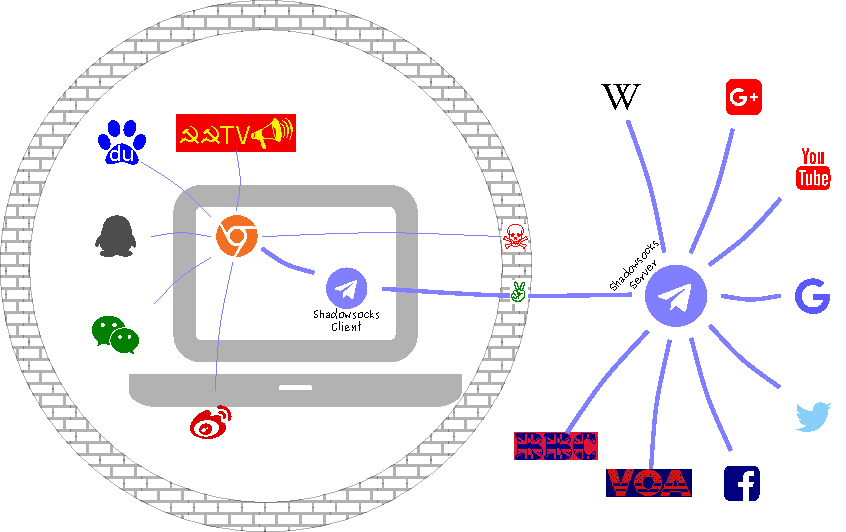
\includegraphics[width=.8\linewidth]{./ss-img.pdf}
\end{center}

There are Shadowsocks client software for all the main stream operating systems, including
MS-Windows, all desktop Linux, Android, MAC OSX, iOS. Here I only give you a brief
introduction on how to setup and use it in the Debian GNU/Linux\footnote{\url{https://www.debian.org}} system which is my
favorite.

What you need besides Debian:
\begin{enumerate}
\item A Shadowsocks client software.
\item A Google Chrome web browser with a proxy extension installed.
\item A Shadowsocks server. There are some free (and usually not so stable) servers can be
found on the web; There are also a lot of paid Shadowsocks services available for
approximately 100RMB/year; And also you can buy cloud service, e.g. \href{https://cloud.google.com}{Google cloud}\footnote{\url{https://cloud.google.com}}, and
then install your own Shadowsocks server on your own cloud. Whatever, you have to
manage to get a server yourself, otherwise you can't setup a working Shadowsocks link.
\end{enumerate}

\section{Shadowsocks client installation}

\begin{verbatim}
    sudo apt update
    sudo apt install shadowsocks-libev
\end{verbatim}
Easy, eh?

\section{Shadowsocks client configuration}

Example config file: \texttt{/etc/shadowsocks-libev/config.json}

\begin{minted}[mathescape=true,linenos=true,numbersep=5pt,frame=lines,framesep=2mm]{javascript}
{
    "server":"127.0.0.1",
    "server_port":8388,
    "local_port":1080,
    "password":"fuPodNics",
    "timeout":60,
    "method":"chacha20-ietf-poly1305"
}
\end{minted}

Line by line explanation:
\begin{enumerate}
\item Left curly bracket indicates the beginning of the config file;
\item The IP address, or the domain name, of the Shadowsocks server. Remember? You have to
find a server yourself, either a free one or a paid service;
\item The port number used by the server. A connection will be setup between your local port
(usually port 1080) and this server port;
\item The port number of the client you just installed. Usually it's 1080. Your web browser
will pass all the data to this port of your client. Then your client will encrypt
the data and send it to the server port through the ready-setup Shadowsocks
connection;
\item The password needed when your client accesses the server;
\item Timeout if the client can't connect to the server in 60 seconds;
\item The encryption method to be used by the server;
\item Right curly bracket indicates the end of the configuration.
\end{enumerate}

If you have more than one server to use, you have to write a config file for each
server. And you can only use one at a time. For example, assuming you have two config
files (\texttt{a.json}, and \texttt{b.json}) in your \texttt{/etc/shadowsocks-libev/} directory, and 
you started a Shadowsocks process by using the following command:
\begin{verbatim}
    ss-local -v -c /etc/shadowsocks-libev/a.json
\end{verbatim}
Sometime later, you see a lot of screen output like the following:
\begin{footnotesize}
\begin{verbatim}
    2018-08-31 19:37:50 ERROR: server_recv_cb_recv: Connection reset by peer
    2018-08-31 19:37:50 ERROR: server_recv_cb_recv: Connection reset by peer
    2018-08-31 19:37:50 ERROR: server_recv_cb_recv: Connection reset by peer
    2018-08-31 19:37:50 ERROR: server_recv_cb_recv: Connection reset by peer
    2018-08-31 19:37:50 ERROR: server_recv_cb_recv: Connection reset by peer
\end{verbatim}
\end{footnotesize}
This indicates the connection is gone. Then you can switch to \texttt{b.json} by:
\begin{enumerate}
\item Typing \texttt{Ctrl-c} to stop the current Shadowsocks process;
\item Starting a new process by:
\begin{verbatim}
ss-local -v -c /etc/shadowsocks-libev/b.json
\end{verbatim}
\end{enumerate}

\section{Google Chrome extension installation and configuration}
\label{sec:org856d758}
The extension we need is \href{https://chrome.google.com/webstore/detail/proxy-switchyomega/padekgcemlokbadohgkifijomclgjgif?utm\_source=chrome-ntp-icon}{\emph{Proxy Switchy Omega}}\footnote{\url{https://chrome.google.com/webstore/detail/proxy-switchyomega/padekgcemlokbadohgkifijomclgjgif?utm\_source=chrome-ntp-icon}}. It can help you easily switch on/off the
proxy. It's not strictly mandatory. Without it, you can bypass the GFW like this:
\begin{verbatim}
    ss-local -v -c /etc/shadowsocks-libev/b.json
    google-chrome --proxy-server='socks5://127.0.0.1:1080'
\end{verbatim}
But in this way, you cannot switch the proxy off even when you visit \href{https://baidu.com}{baidu.com}\footnote{\url{https://baidu.com}}.

Usually, the Chrome extensions can only be installed via \href{https://chrome.google.com/webstore/category/extensions?utm\_source=chrome-ntp-icon}{Chrome Web Store}\footnote{\url{https://chrome.google.com/webstore/}}. Unluckily, it's
blocked by YOU KNOW WHO. So you can use the above two commands to visit Chrome Web Store,
and install the Proxy Switchy Omega extensions.

After successfully installed \emph{Proxy Switchy Omega}, you should close your Google Chrome
window, and then re-open it, by typing just \texttt{google-chrome} without followed by any
options. At the upper right corner of the browser window, you should find the circle
logo of \emph{Proxy Switchy Omega}. Now it's time to configure it.
A picture is worth a thousand words, right?

\begin{center}
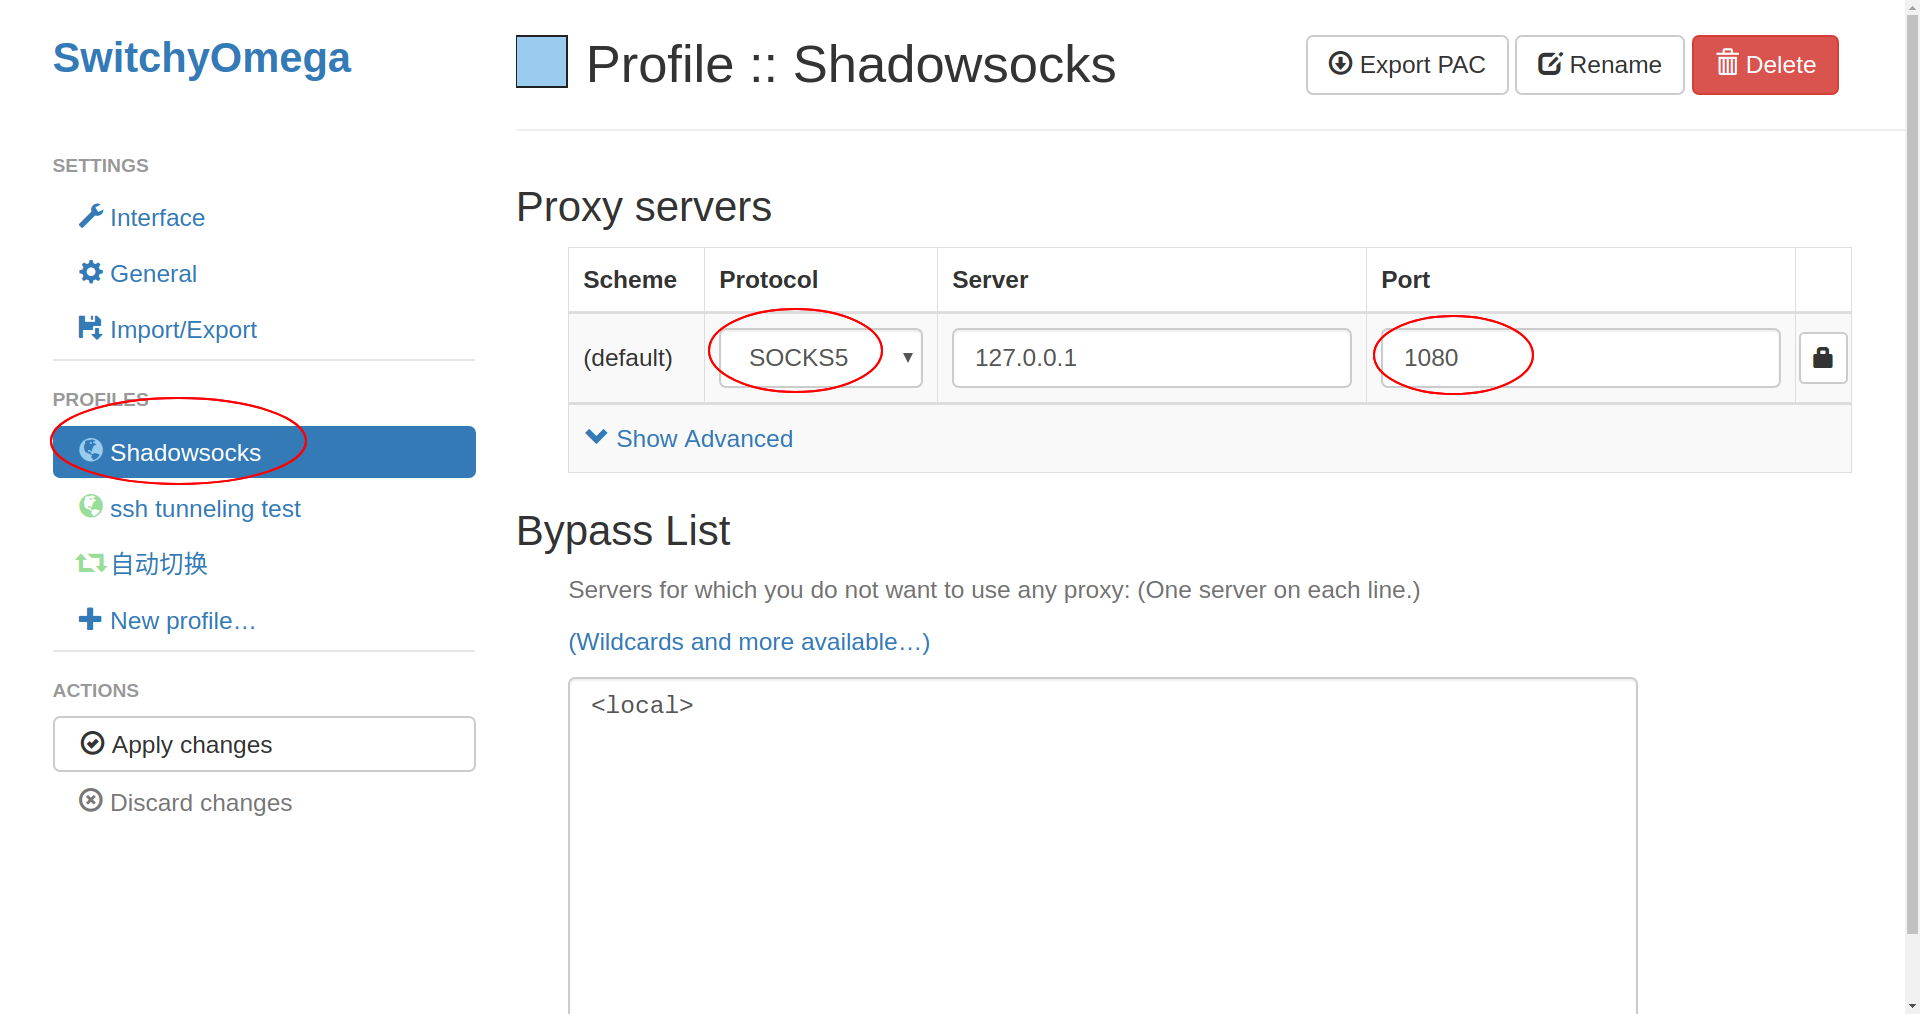
\includegraphics[width=.8\linewidth]{./switchyomega1.png}
\end{center}
And \emph{Proxy Switchy Omega} needs a set of rule to decide when to trigger the Shadowsocks
proxy on/off. You can find a ready-to-use rule set \href{https://github.com/shminer/SwitchyOmega-backup}{here}\footnote{\url{https://github.com/shminer/SwitchyOmega-backup}}. 

Summary:
\begin{enumerate}
\item Start your local Shadowsocks agent first:
\begin{verbatim}
    ss-local -v -c /etc/shadowsocks-libev/b.json
\end{verbatim}
\item configure \emph{Proxy Switchy Omega}, and usually put it in \emph{auto switch} mode.
\end{enumerate}


Enjoy hacking!
\end{document}
%%% Local Variables:
%%% mode: latex
%%% TeX-master: t
%%% End:
